\documentclass[a4paper,10pt]{article}
\usepackage[utf8]{inputenc}

\usepackage[english]{babel}
\usepackage[dvinames]{xcolor}
\usepackage[compact,small]{titlesec}
\usepackage{booktabs}
\usepackage{multirow}
\usepackage{amsfonts,amsmath,amssymb}
\usepackage{marginnote}
\usepackage[top=1.8cm, bottom=1.8cm, outer=1.8cm, inner=1.8cm, heightrounded, marginparwidth=2.5cm, marginparsep=0.5cm]{geometry}
\usepackage{enumitem}
\setlist{noitemsep,parsep=2pt}
\newcommand{\highlight}[1]{\textcolor{kuleuven}{#1}}
\usepackage{pythonhighlight}
\usepackage{cleveref}
\usepackage{graphicx}
\usepackage{algorithm}
\usepackage{algpseudocode}

\newcommand{\nextyear}{\advance\year by 1 \the\year\advance\year by -1}
\newcommand{\thisyear}{\the\year}
\newcommand{\deadlineCode}{December 31, \thisyear{} at 16:00 CET}
\newcommand{\deadlineReport}{\deadlineCode}

\newcommand{\ReplaceMe}[1]{{\color{blue}#1}}
\newcommand{\RemoveMe}[1]{{\color{purple}#1}}

\setlength{\parskip}{5pt}

%opening
\title{Evolutionary Algorithms: Final report}
\author{Jorrit Willaert (r0652971)}

\begin{document}
\fontfamily{ppl}
\selectfont{}

% TODO Add bold keywords

\maketitle

\section{Metadata}

\begin{itemize}
 \item \textbf{Group members during group phase:} Lukas De Greve and Thomas Vanhemel
 \item \textbf{Time spent on group phase:} \ReplaceMe{10 hours}
 \item \textbf{Time spent on final code:} \ReplaceMe{50 hours}
 \item \textbf{Time spent on final report:} \ReplaceMe{13 hours}
\end{itemize}

\section{Peer review reports (target: 1 page)}

\subsection{The weak points}
\begin{enumerate}
 \item Our initial recombination operator was a \textbf{simplified version of the edge crossover operator} \cite{initial_implementation_edge_crossover}. This version did not prioritize common edges between parents, but only chose an entry which itself had the shortest list. Hence, not enough exploitation of the parents features followeds. 
 \item The ($\kappa$ + $\mu$)-elimination (without any type of diversity promotion) puts a \textbf{lot of selective pressure} on the population.
 \item Our \textbf{mutation operator does not scale} to larger problems, since it only swaps two random locations. As a consequence, the mutation operator will have an even smaller impact on the solution when the problem size increases. 
 \item Due to the elimination strategy, together with the chosen mutation operator, \textbf{premature convergence} was observed.
\end{enumerate}

\subsection{The solutions}
\begin{enumerate}
 \item The simplified version of the edge crossover operator was first replaced with the \textbf{proper edge crossover operator} \cite{eiben_smith}. However, once the running times of edge recombination were compared with the ones of order crossover, it was apparent that \textbf{order crossover} was much faster. For this reason, edge crossover was abandoned in favor for order crossover.
 \item The ($\kappa$ + $\mu$)-elimination was kept for quite some time, but was supplemented with \textbf{fitness sharing}. The high selective pressure of ($\kappa$ + $\mu$)-elimination was therefore largely mitigated with the introduction of this diversity promotion scheme. However, to further reduce the selective pressure present in the ($\kappa$ + $\mu$)-elimination, the operator was swapped for the \textbf{k-tournament elimination} operator in the final version of the algorithm (along with the same fitness sharing technique).
 \item The mutation operator has been changed from swap mutation to \textbf{inversion mutation}. Hence, the effect of the mutation operator is constant for rising problem sizes.
 \item With the introduction of fitness sharing, along with the inversion mutation operator, \textbf{premature convergence} was largely \textbf{avoided}.
\end{enumerate}

\subsection{The best suggestion}
Both groups suggested to modify the simplified edge crossover operator to the `proper' one. Although this certainly is a useful suggestion, another suggestion by one group is even more useful in my opinion, given that I was going to change the crossover operator in the individual phase anyway. The other suggestion is about changing the mutation operator from swap mutation to inversion mutation. In the group phase part of the project, we hadn't really observed the shortcoming of the swap mutation, which only became clear after their suggestion has been made.

\section{Changes since the group phase (target: $0.5$ pages)} 
\begin{enumerate}
\item The simplified edge recombination operator was first replaced with the \textbf{proper edge recombination operator}, after which it eventually was replaced by the \textbf{order recombination operator} due to massive speed gains. An elaboration on the recombination operators is provided in Section \ref{recombination}. 
\item \textbf{Fitness sharing} has been introduced in the elimination step, as further explained in Section \ref{diversity_promotion}.
\item A \textbf{local search operator} (2-opt) has been introduced to increase the fitnesses of the newly created offsprings (Section \ref{local_search_operator}).
\item Simple random initialization has been replaced by \textbf{greedy} and \textbf{legal initialization}, as further explained in Section \ref{initialization}.
\item The mutation operator has been changed from the swap mutation to \textbf{inversion mutation}. This is more elaborated in Section \ref{mutation}.
\item The elimination operator has eventually been changed from ($\kappa$ + $\mu$)-elimination to \textbf{k-tournament elimination}, for reasons explained further in Section \ref{elimination}.
\item Numerous \textbf{optimizations} have been made in almost all parts of the algorithm to significantly increase the execution speed.
\end{enumerate}

\section{Final design of the evolutionary algorithm (target: $3.5$ pages)} 
\subsection{The three main features}
\begin{enumerate}
\item \textbf{Fitness sharing} has been used in the elimination step of the algorithm. This diversity promotion scheme is of crucial importance to \textbf{avoid premature convergence}, and hence makes sure that far better solutions can be found, instead of letting all individuals converge to one local minima.
\item By introducing the 2-opt \textbf{local search operator}, far better solutions were found more quickly. Without the local search operator, much more iterations were required to find the same fitness values, along with a necessarily larger population. Although this operator is inherently extremely computationally expensive, it is turns out to be pivotal for the algorithm. Especially in this operator, optimizations such as making use of \textbf{dynamic programming} and using \textbf{Numba} were decisive in making the operator computationally feasible.
\item One last crucial improvement is the introduction of the \textbf{greedy} and \textbf{legally initializations}. Greedy initialization starts from a random node, and chooses the next one according to the smallest distance. The details of this initialization scheme are elaborated in Section \ref{initialization}, along with a consideration of the introduced biases. Furthermore, legal initialization simply chooses the next node from a random neighbor that has an existing road between them.
\end{enumerate}

\subsection{The main loop}

\ReplaceMe{Make a picture of the ``flow'' in your evolutionary algorithm, similar to the example below. Include all the main components (mutation, recombination, selection, elimination, initialization, local search operators, diversity promotion mechanisms). There are no formal requirements on how to do this, as long as it is clear and you can efficiently explain your complete evolutionary algorithm using this picture at the exam. Contrary to the picture below, include the specific techniques, e.g., top-$\lambda$ elimination, $k$-tournament selection, where possible.}

% TODO

%
%\begin{center}
%\includegraphics[height=10em]{../../BasicLoop.png}
%\end{center}

\clearpage
\subsection{Representation}
Possible solutions are represented as \textbf{permutations} and are written down in \textbf{cycle notation}. E.g. the permutation (1423) starts at node 1, then goes to 4, then 2, then 3, and returns to 1. An advantage of this notation is that no cycles are present as long as we initialize the representations as a permutation of all nodes. 

This representation is implemented in our program as a Numpy array with length equal to the number of nodes in the problem. Each element in the array consists of one integer number: the node number.

\subsection{Initialization}
\label{initialization}
In the group-phase part of the project, individuals were generated by a \textbf{random permutation}, with their size determined from the distance matrix. However, especially for the larger problem sizes, quite a lot of paths were \textbf{nonexisting} or \textbf{extremely long}. Hence, random initialization of all individuals yielded almost always individuals where none of them represented a valid path. 

Two new initialization schemes were introduced, legal and greedy initialization, where the objective of legal initialization is to not create impossible paths when initialing an individual. This while not introducing certain biases, such as individuals who take over the population immediately. The objective of greedy initialization is introducing locally optimal individuals with a high fitness, in a computationally inexpensive way. Here, special care has been taken that the individuals don't introduce high biases and won't take over the population immediately.

\subsubsection{Legal initialization}
When initializing an individual legally, one makes sure that the generated path \textbf{exists}. Therefore, a city is chosen at random, after which the next city in the tour is chosen to be a random one out of all the neighbors with a non-infinite path cost. If, however, no existing neighbors are available anymore as next cities, the whole procedure restarts. The pseudo-algorithm is given in Algorithm \ref{legal_initialization_algorithm}.

\begin{algorithm}
\caption{Legal initialization}\label{legal_initialization_algorithm}
\begin{algorithmic}
\While {True}
\State Choose the initial city at random
\While {individual not entirely generated}
\State Generate all legal possibilities
\If {no legal possibilities}
\State Break out of inner loop
\EndIf
\State Choose a random city to be the successor of the previous city
\EndWhile
\If {not broken out of inner loop and path from the last city to the first one is not infinity}
\State Return newly generated individual
\EndIf
\EndWhile
\end{algorithmic}
\end{algorithm}

This legal initialization scheme \textbf{does not introduce undesirable biases}. In theory, also the most optimal route could have been initialized, and the only bias present is a bias to not have nonexisting paths. I therefore can't think of any disadvantage this initialization scheme entails. 

\subsubsection{Greedy initialization}
\label{greedy_initialization}
Besides the legal initialization scheme, I also initialize some individuals greedily. The algorithm resembles the legal initialization scheme, with the only change that the successor city is chosen to be the \textbf{closest neighbor}, instead of a random legal neighbor. The pseudo-algorithm is given in Algorithm \ref{greedy_initialization_algorithm}.

\begin{algorithm}
\caption{Greedy initialization}\label{greedy_initialization_algorithm}
\begin{algorithmic}
\While {True}
\State Choose the initial city at random
\While {individual not entirely generated}
\State Generate all legal possibilities
\If {no legal possibilities}
\State Break out of inner loop
\EndIf
\State Choose the closest neighboring city to be the successor of the previous city
\EndWhile
\If {not broken out of inner loop and path from the last city to first one is not infinity}
\State Return newly generated individual
\EndIf
\EndWhile
\end{algorithmic}
\end{algorithm}

This initialization scheme \textbf{does introduce certain biases}, which could result in some individuals taking over the population immediately. Therefore, one has to take preventions against this bias, by for example only initializing a small fraction of all the individuals with this scheme, as could be observed in the chosen hyperparameters of Section \ref{general_aspects_initialization}.

The introduced bias is that all individuals are locally optimal, where in theory the maximum number of different solutions is given by the problem size. Given that it may be difficult to escape local minima, one must consider the usefulness of this initialization scheme.

However, after experimenting with this initialization scheme, it became apparent that \textbf{good solutions} for the problem where found much faster, while still \textbf{maintaining a lot of diversity}, along with a \textbf{smooth convergence}. With only a small portion of the individuals being initialized with this scheme, being totally stuck in a local minima was not observed, and for me it brought huge advantages, since the given five minutes could now be used to start searching in some way more interesting regions of the search space.

\subsubsection{General aspects}
\label{general_aspects_initialization}
The distance matrix can be given in such a way that greedy initialization gets stuck in an \textbf{infinite loop}, because greedy initialization simply constructs a dead path (due to always taking the closest neighbor), starting from each node. To create a legal path in special cases, it should instead sometimes take sub-optimal paths to a neighbor to not end up in a dead path near the end of the initialization. To prevent the whole algorithm from crashing, a \textbf{time constraint} on the initialization of one individual has been introduced. Once an individual takes longer than two second to initialize, simple random initialization of that individual ensues.

An individual also gets assigned a random $\alpha$ value, which represents the probability that the individual will mutate in the mutation step of the algorithm. This way, a suitable mutation rate is determined by \textbf{self-adaptivity}.

The initial value of $\alpha$ is given by Formula \ref{initial_alpha}.

\begin{equation}
    \label{initial_alpha}
    \alpha = max(0.01, 0.05+0.02 \cdot (X \sim \mathcal{N}(0,\,1)))
\end{equation}

After some testing with population sizes, a size of 15 has been chosen. Furthermore, as mentioned in Section \ref{greedy_initialization}, only a fraction of the population should be initialized greedily. Given that the  population size is 15, I found that greedily initializing 20 \% of the individuals (i.e. 3 individuals) worked out quite well in practice. The remaining 80 \% of the individuals are initialized legally.

For large problem sizes, initialization could take up to 10 seconds. Since the initialization of an individual is totally independent of the other individuals, \textbf{multiprocessing} has been added to this step, which entailed a factor five speed improvement on a machine with four physical cores (eight virtual cores).


\subsection{Selection operators}
\label{selection}
The \textbf{k-tournament selection operator} from the group phase part has been kept. This selection operator is computationally inexpensive, since only k fitness values have to be computed, while this would require $\mu$ fitness values in fitness-based methods. Furthermore, sigma-scaled selection would for example not have been an appropriate choice, since the greedy initialization scheme introduces some very good individuals in the population. These individuals would dominate, since their selection probability would be very high.

A k-value of 5 has been chosen after numerous experiments.

\subsection{Mutation operators}
\label{mutation}
The mutation operator used for the final implementation is the \textbf{inversion mutation}, whereby a random sub-vector is chosen and its order is reversed. The swap mutation operator that was used in the group phase part, did not scale well to larger problems, since it only swaps two random locations. That mutation operator, as a consequence, had a relatively even smaller impact on the solution when the problem size increased.

Inversion mutation does not suffer from this scaling problem, since the cities that determine the sub-vector are randomly chosen. Hence, the effect of the mutation operator is constant for rising problem sizes.  

Self-adaptivity has been used for the mutation rate, which is hence specific to each individual, and is initialized as in Formula \ref{initial_alpha}, which changes in crossover as described in Formula \ref{crossover_alpha_1} and Formula \ref{crossover_alpha_2}.

\begin{equation}
    \label{crossover_alpha_1}
    \beta = 2 \cdot (X \sim \mathcal{N}(0,\,1) - 0.5
\end{equation}

\begin{equation}
    \label{crossover_alpha_2}
    alpha = max(0.01, \alpha_{parent\_1} + \beta \cdot (\alpha_{parent\_2} - \alpha_{parent\_1})
\end{equation}

\subsection{Recombination operators}
\label{recombination}
%\ReplaceMe{Which recombination operators did you implement? If they are not from the slides, describe them. How do you choose among several recombination operators? Why did you choose these ones specifically? Explain how you believe that these operators can produce offspring that combine the best features from their parents. How does your operator behave if there is little overlap between the parents? Can your recombination be controlled with parameters; what behavior do they change? Do you use self-adaptivity? Do you use any other advanced parameter control mechanisms (e.g., variable across iterations)? Did you try other recombination operators not included in the final version? Why did you discard them? Did you consider recombination with arity strictly greater than 2?}

In the group phase part of the project, a \textbf{simplified version} of the \textbf{edge crossover operator} was used as the recombination algorithm, for which the process is described in Algorithm \ref{simple_edge_crossover} \cite{initial_implementation_edge_crossover}. This recombination results in a new path where all edges of the child were present in at least one of the parents. It does however not prioritize edges present in both parents over edges present in a single parent.

\begin{algorithm}
\caption{Simple edge recombination operator}\label{simple_edge_crossover}
\begin{algorithmic}
\State Let K be the empty list
\State let N be the first node of a random parent
\While{length(K) $<$ length(Parent)}
\State Append N to K
\State Remove N from all neighbor lists
\If{N's neighbor list is not empty}
\State let $N^*$ be the neighbor of N with the fewest neighbors in its list (or a random one, in case of multiples)
\Else 
\State let $N^*$ be a randomly chosen node that is not in K
\EndIf
\State N $\gets N^*$
\EndWhile
\end{algorithmic}
\end{algorithm}

This algorithm is very simple and was the weakest part of the genetic algorithm. However, the algorithm still has some desirable features despite its simplicity. When N consecutive edges are present in both parents (N $ \ge $ 2), the child will contain at least N/2 of these edges, so important features are mostly preserved. On the other hand,
when the parents are very different, the child will look fairly different from both parents. This combined with some aspects of randomness in the algorithm makes it decent at exploring the different solutions. 

The reason this simplified algorithm was implemented, instead of the proper one from Eiben \& Smith \cite{eiben_smith}, was due to the belief that the computational cost of this algorithm was (much) lower than the one from Eiben \& Smith. 

For the individual phase of the project, an analysis was made between order crossover and the proper edge crossover algorithm of Eiben \& Smith. After some research, with a lot of contradictory advices, an arbitrary choice has been made to first try out the \textbf{proper edge crossover algorithm}.

Implementation wise, quite a lot of effort has been made to catch all the corner cases of the algorithm, along with achieving relatively optimized code. The algorithm was kept a long time thereafter, until it was noticed that for the large problem sizes, crossover took an \textbf{extremely long time} (up to 95 \% of the total runtime was spend in the edge crossover operator).

\begin{algorithm}
\caption{`Proper' edge recombination operator \cite{eiben_smith}}\label{proper_edge_crossover}
\begin{algorithmic}
\State Construct the edge table
\State Pick an initial element at random and put it in the offspring
\While {the offspring is not entirely constructed}
\State Set the variable $current\_element = entry$
\State Remove all references to $current\_element$ from the table
\If {there is a common edge}
\State Pick that to be the next one
\Else
\State Pick the entry in the list which itself has the shortest list (split ties at random)
\EndIf
\If {an empty list is reached}
\If {the other end has not yet been examined}
\State Examine the other end for extension
\Else
\State Choose a new element at random
\EndIf
\EndIf
\EndWhile
\end{algorithmic}
\end{algorithm}

Due to this slow execution time, \textbf{order crossover} \cite{eiben_smith} has been implemented as well (Algorithm \ref{order_crossover_algorithm}).

\begin{algorithm}
\caption{Order crossover operator \cite{eiben_smith}}\label{order_crossover_algorithm}
\begin{algorithmic}
\State Choose two crossover points at random
\State Copy the segment between them from the first parent into the offspring
\State Starting from the second crossover point in the second parent, copy the remaining unused numbers into the child in the order they appear in the second parent, wrapping around at the end of the list.
\end{algorithmic}
\end{algorithm}

This crossover algorithm is inherently much cheaper to calculate and takes only about 5 \% of the total execution time in the final algorithm. This is exactly the reason why this crossover algorithm was eventually used. 

In hindsight, one reason for the slow execution time of the edge crossover operator is probably due to the usage of sets in the operator. The edge table was basically one list with sets, where a minus denoted a double entry. Sets were used because it was desirable to check quickly if an edge was present in the edge table. However, since for each element, maximum four edges could be present, lists would probably have sufficed. The same reasoning applies because quite some bookkeeping was required with the sets (e.g. deleting a positive entry if it occurred for the second time, to insert it afterwards with a minus in front of it). 

Another reason for the big performance gap is the fact that the order crossover operator was able to use \textbf{Numba} for compiling the Python code and running it way faster, by using the decorator $@jit(nopython=True)$. This because the order crossover operator only uses operations on Numpy arrays (which Numba handles perfectly well), while Numba threw hundreds of compile errors in the edge crossover method, because Numba (in the $nopython=True$ mode) couldn't create new Numpy arrays, had difficulties with working on sets, and wasn't able to infer the $dtype$'s most of the time.

% TODO say how you get new alpha value

\subsection{Elimination operators}
\label{elimination}
%\ReplaceMe{Which elimination operators did you implement? If they are not from the slides, describe them. Why did you select this one? Are there parameters that need to be chosen? Did you use an advanced scheme to vary these parameters throughout the iterations? Did you try other elimination operators not included in the final version? Why did you discard them?}
For a long time, the \textbf{($\kappa$ + $\mu$)-elimination} from the group phase part was kept in the algorithm. However, for the smaller problem sizes, it was noted that the population converged extremely quickly, even with the fitness promotion scheme present (as further discussed in Section \ref{diversity_promotion}). After some research, it became apparent that the ($\kappa$ + $\mu$)-elimination operator actually puts quite a lot of selective pressure. A \textbf{k-tournament operator}, in contrast, can mitigate this selective pressure, hence the ($\kappa$ + $\mu$)-elimination operator has been exchanged for the k-tournament operator.

To combine the k-tournament operator with the fitness sharing operator, Algorithm \ref{elimination_algorithm} is for the k-tournament operator (along with some preparatory computations), while Algorithm \ref{fitness_sharing_algorithm} is invoked each time for the fitness sharing diversity promotion scheme itself.

\begin{algorithm}
\caption{Elimination \cite{eiben_smith}}\label{elimination_algorithm}
\begin{algorithmic}
\State Calculate the fitnesses for all the individuals
\State Add the best individual to the list `survivors'
\For{i from 0 to $\lambda - 2$}
\State Calculate the new fitness values, based on fitness sharing
\For{j from 0 to $k_{elimination} - 1$}
\State Randomly sample a fitness value (`fit') from the new list of fitness values
\If{`fit' is the lowest fitness found}
\State Store the index of the individual that corresponds to this fitness under `idx'
\EndIf
\EndFor
\State The new survivor is the individual located at `idx'
\State Append the new survivor to the `survivors' list
\State Delete the survivor from the list containing all the individuals
\EndFor
\end{algorithmic}
\end{algorithm}

After numerous experiments, a k-value of 8 has been chosen.

\subsection{Local search operators}
\label{local_search_operator}
%\ReplaceMe{What local search operators did you implement? Describe them. Did they cause a significant improvement in the performance of your algorithm? Why (not)? Did you consider other local search operators that did not make the cut? Why did you discard them? Are there parameters that need to be determined in your operator? Do you use an advanced scheme to determine them (e.g., adaptive or self-adaptive)?}
The \textbf{2-opt local search operator} has been implemented, which swaps every two possible edges in a given cycle. In a first version of this algorithm, the fitness was recalculated for every possible neighbor of the given individual, which entailed an unacceptable high computational cost, especially for the larger problem sizes. After some investigation, patterns were detected in the computation of the fitness. Hence, instead of recalculating the fitness for every neighbor, some kind of \textbf{dynamic programming} approach was undertaken. For every individual, there is a sort of preprocessing step, whereby so-called `cumulatives' are created. These cumulatives capture the path length from the first city to that corresponding city in the cumulative array. The same process applies for the calculation of the path length from the last city to the corresponding city in the array (i.e. in reverse order, whereby the return cost of the last city to the first city is also incorporated). It is clear that the calculation of these cumulatives is done in $O(N)$, where $N$ is the number of cities in the problem size.

Now, calculations of fitnesses of individuals are simply a matter of bookkeeping. The process is explained in Algorithm \ref{local_search_operator_algorithm}.

% TODO maybe explain the loops a bit in words as well

\begin{algorithm}
\caption{Local search operator}\label{local_search_operator_algorithm}
\begin{algorithmic}
\State Let the best fitness be the fitness of the original individual
\State Let the best combination be (0, 0)
\State Build cumulatives
\For {first from 1 to (length - 3)} 
\State $fit_{first \; part} = forward\_cumulative[first - 1]$
\State $fit_{middle \; part} = 0.0$
\For {second from (first + 2) to (length - 1)}
\State $fit_{middle \; part} \mathrel{{+}{=}} distanceMatrix[order[second-1]][order[second-2]]$
\State $fit_{last \; part} = backward\_cumulative[second]$
\State $first\_bridge = distanceMatrix[order[first-1]][order[second-1]]$
\State $second\_bridge = distanceMatrix[order[first]][order[second]]$
\State $fitness = fit_{first \; part} + first\_bridge + fit_{middle \; part} + second\_bridge + fit_{last \; part}$
\If {$fitness < best\_fitness$}
\State Let the new best combination be (first, second)
\State Let the new best fitness be the newly calculated fitness
\EndIf
\EndFor
\EndFor
\State Swap the order of the individual from the best first to the best second, obtained from the best combination.
\end{algorithmic}
\end{algorithm}

As further illustrated in Figure \ref{local_search_operator_2_opt}, the first part of the tour is simply the same as the previous iteration, with one extra cost added from `first - 1' to `first'. The same reasoning applies for the last part of the tour, where in this case the total cost decreases each time by the cost from `second - 1' to `second'. Finally, also the middle part can be build up in an analogous way. This way, the total cost of the 2-opt local search algorithm is only ($O(N^2)$, where $N$ denotes the total number of cities. 

\begin{figure}[H]
\caption{Local search operator (2-opt) \cite{local_search_slides}}
\label{local_search_operator_2_opt}
\centering
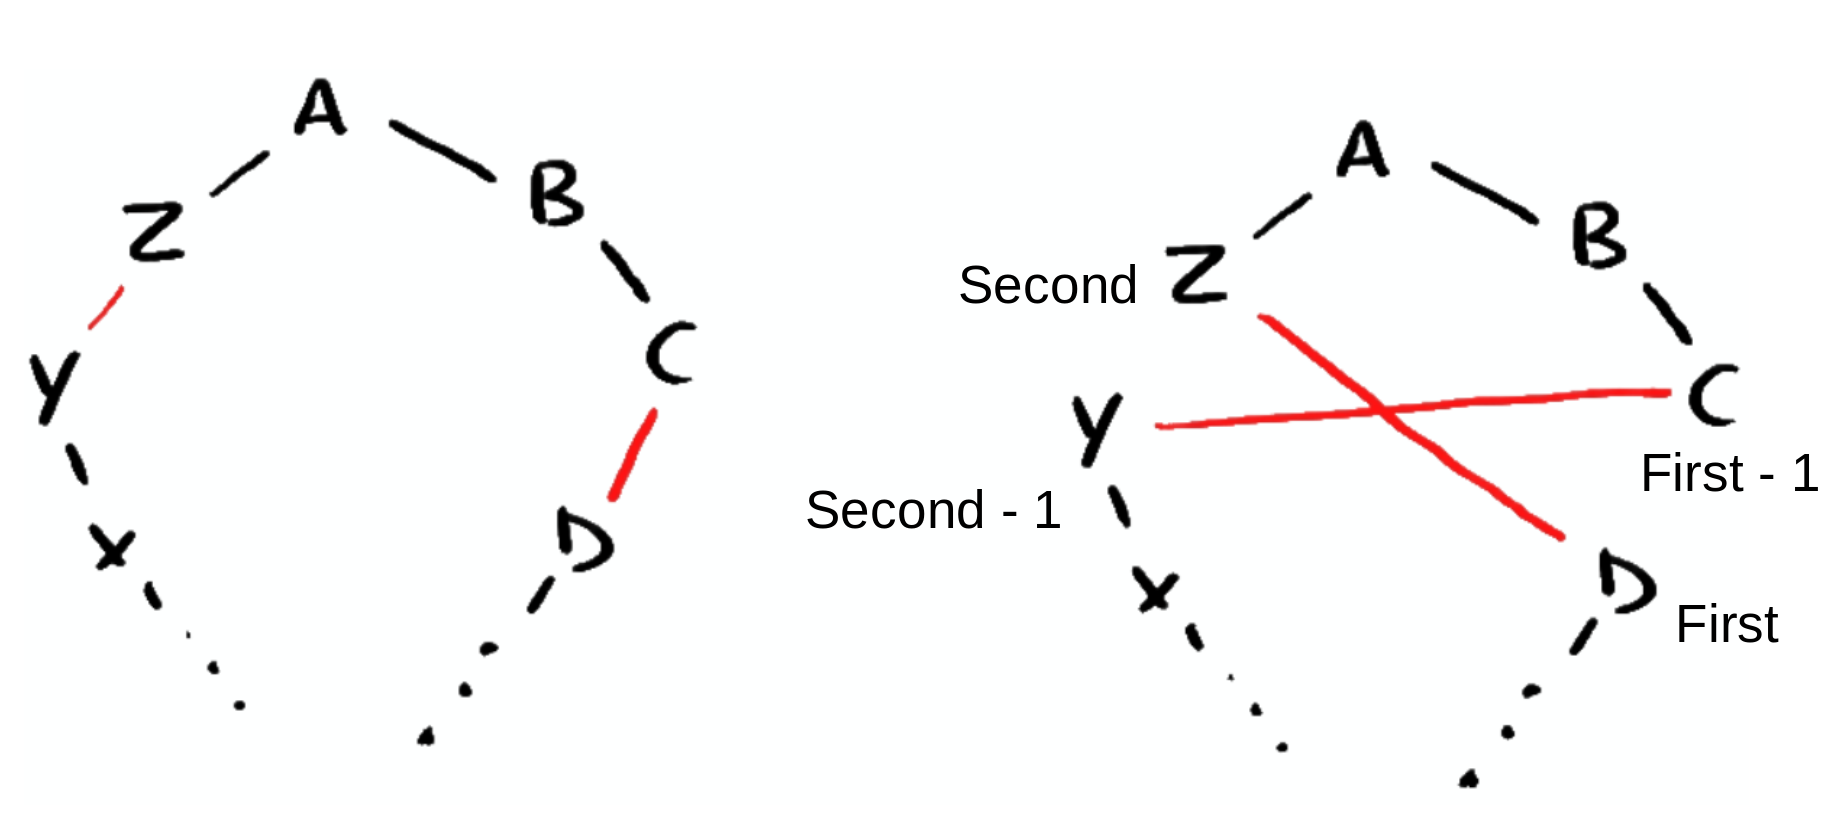
\includegraphics[width=0.4\textwidth]{local_search_operator_2_opt.png}
\end{figure}

It should also be noted that by using Numba with the command $@jit(nopython=True)$ above the method declarations, the local search operator runs \textbf{745 times as fast}. Numba can make these huge improvements due to compilation of these methods, where especially the loops can be exploited.

\subsection{Diversity promotion mechanisms}
\label{diversity_promotion}
\ReplaceMe{Did you implement a diversity promotion scheme? If yes, which one? If no, why not? Describe the mechanism you implemented. In what sense does the mechanism improve the performance of your evolutionary algorithm? Are there parameters that need to be determined? Did you use an advanced scheme to determine them?}

\begin{algorithm}
\begin{algorithmic}
\label{fitness_sharing_algorithm}
%TODO
\State TODO
\end{algorithmic}
\end{algorithm}

\subsection{Stopping criterion}
Not a lot of effort has been put in implementing a stopping criterion, since all the larger problems stayed converging after running for five minutes. Hence, the stopping criterion is simply the time limit of five minutes.

% TODO maybe some other stopping criterion?
\ReplaceMe{Which stopping criterion did you implement? Did you combine several criteria?}

\subsection{Parameter selection}

\ReplaceMe{For all of the parameters that are not automatically determined by adaptivity or self-adaptivity (as you have described above), describe how you determined them. Did you perform a hyperparameter search? How did you do this? How did you determine these parameters would be valid both for small and large problem instances?}

\begin{enumerate}
    \item The population size = 15
    \item The offspring size = 15
    \item The k-tournament parameter of the selection operator = 5 
    \item The k-tournament parameter of the elimination operator = 8
    \item The $\alpha$-value of fitness-sharing = 0.25
    \item The $\sigma$-value of fitness-sharing = half of the problem size
\end{enumerate}

\subsection{Other considerations}

% TODO hashmaps for fitnesses
% Elitism

\ReplaceMe{Did you consider other items not listed above, such as elitism, multiobjective optimization strategies (e.g., island model, pareto front approximation), a parallel implementation, or other interesting computational optimizations (e.g. using advanced algorithms or data structures)? You can describe them here or add additional subsections as needed.}


\section{Numerical experiments (target: 1.5 pages)}

\RemoveMe{\textbf{Goal:} Based on this section and our execution of your code, we will evaluate the performance (time, quality of solutions) of your implementation and your ability to interpret and explain the results on benchmark problems.}

\subsection{Metadata}

\ReplaceMe{What parameters are there to choose in your evolutionary algorithm? Which fixed parameter values did you use for all experiments below? If some parameters are determined based on information from the problem instance (e.g., number of cities), also report their specific values for the problems below.

Report the main characteristics of the computer system on which you ran your evolutionary algorithm. Include the processor or CPU (including the number of cores and clock speed), the amount of main memory, and the version of Python 3.}
These experiments were conducted on an Intel Core i7-6700HQ CPU, with a clock frequency of 3.60GHz and 8 virtual cores. The systems contains 16 GB of main memory, and Python version 3.8 was used for the tests.

\subsection{tour29.csv}

\ReplaceMe{Run your algorithm on this benchmark problem (with the 5 minute time limit from the Reporter). Include a typical convergence graph, by plotting the mean and best objective values in function of the time (for example based on the output of the Reporter class). 

What is the best tour length you found? What is the corresponding sequence of cities? 

Interpret your results. How do you rate the performance of your algorithm (time, memory, speed of convergence, diversity of population, quality of the best solution, etc)? Is your solution close to the optimal one?

Solve this problem 1000 times and record the results. Make a histogram of the final mean fitnessess and the final best fitnesses of the 1000 runs. Comment on this figure: is there a lot of variability in the results, what are the means and the standard deviations?}

\subsection{tour100.csv}

\ReplaceMe{Run your algorithm on this benchmark problem (with the 5 minute time limit from the Reporter). Include a typical convergence graph, by plotting the mean and best objective values in function of the time (for example based on the output of the Reporter class). 

What is the best tour length you found in each case? 

Interpret your results. How do you rate the performance of your algorithm (time, memory, speed of convergence, diversity of population, quality of the best solution, etc)? Is your solution close to the optimal one?}

\subsection{tour500.csv}

\ReplaceMe{Run your algorithm on this benchmark problem (with the 5 minute time limit from the Reporter). Include a typical convergence graph, by plotting the mean and best objective values in function of the time (for example based on the output of the Reporter class). 

What is the best tour length you found? 

Interpret your results. How do you rate the performance of your algorithm (time, memory, speed of convergence, diversity of population, quality of the best solution, etc)? Is your solution close to the optimal one?}

\subsection{tour1000.csv}

\ReplaceMe{Run your algorithm on this benchmark problem (with the 5 minute time limit from the Reporter). Include a typical convergence graph, by plotting the mean and best objective values in function of the time (for example based on the output of the Reporter class). 

What is the best tour length you found? 

Interpret your results. How do you rate the performance of your algorithm (time, memory, speed of convergence, diversity of population, quality of the best solution, etc)? Is your solution close to the optimal one? }


\section{Critical reflection (target: 0.75 pages)}

\RemoveMe{\textbf{Goal:} Based on this section, we will evaluate your understanding and insight into the main strengths and weaknesses of your evolutionary algorithms.}

\ReplaceMe{What are the three main strengths of evolutionary algorithms in your experience?}

\begin{enumerate}
 \item By using a population-based metaheuristic, a tradeoff can be made between exploration and exploitation. This tradeoff turned out to be instrumental in finding good solutions for the travelling salesman problem. Pure random search is computationally way too expensive (it would even take an infinity before a `decent', simply greedy solution would have been found). Pure local optimizers, on the other hand, would quickly converge to one suboptimal solution, which would most likely also be relatively far from the most optimal solution. Evolutionary algorithms provide a way to find good sub-optimal solutions in a decent amount of time.
 \item Evolutionary algorithms are in principle relatively easy to parallelize, since the population can explore the search space concurrently in many directions. Although in this project, not a lot of parallelization had been used (only in the initialization) step, it would probably be the next most beneficial task to undertake. Trying to use multiprocessing has been undertaken, but the execution time when using multiprocessing was more than a thousand times slower, compared to simple sequential execution on one CPU core. This probably came due to a lot of interprocess communication (IPC), since for example the list of individuals was shared, which resulted in a lot of locks and semiphores, that clearly dominated the execution time.
 \item A last thing that struck me about evolutionary algorithms, is the fact that they in essence optimize a function without using derivatives (only by using the fitness values, leaving aside the local search operator for the moment). Especially for non-differentiable functions may an evolutionary algorithm offer salvation.
\end{enumerate}

\ReplaceMe{What are the three main weak points of evolutionary algorithms in your experience?}

\begin{enumerate}
 \item Evolutionary algorithms work well, as long as they are carefully designed with reasonable parameters. For example, take a population size of 100 instead of 15, and the algorithm struggles to make some iterations. This of course due to the fitness sharing elimination, which has a cubic complexity in terms of the population (and offspring) size. Furthermore, a lot of other parameters have to be chosen to obtain reasonable performance. If for example the k-tournament parameters (from selection and elimination) are not chosen correctly, either the population converges immediately to, or the overall fitnesses of the individuals hardly increase. This, in the end, comes at no surprise, since, according to the no-free-lunch theorem, there cannot exist any algorithm for solving all problems that is generally superior to any competitor.
 \item The representation used in this project clearly yields valuable offsprings after crossover. If one reasons about the representation, it is apparent that subvectors of the parents are probably relatively close to each other, since they come after each other in the tour of the solution. When doing crossover, these \textbf{features} may now be combined in a more optimal way, so the offsprings have clearly a relatively high chance on having a low fitness value as well. However, for a lot of other problems, such representations and crossover operators are not that clear (i.e. features can't be extracted from the parents), and hence evolutionary algorithms can't offer a lot to these problems. 
 \item Evolutionary algorithms are computationally very expensive. Since a lot of exploration is undertaken, inherently a lot of meaningless individuals are constructed while searching.
\end{enumerate}

\ReplaceMe{Describe the main lessons learned from this project. Do you believe evolutionary algorithms are appropriate for the problem studied in this project? Why (not)? What surprised you and why? What did you learn from this project?}
I think that the travelling salesman problem fits perfectly for the project related to this course. Finding an exact solutions is of course infeasible, hence the usage of metaheuristics become necessary and prove themselves to work extremely well. Considering that a lot of real-world applications require good approximations of the optimal solutions, it is obvious that these metaheuristics (and evolutionary algorithms in particular) are an essential tool to possess.

As a side-effect of this course, I would like to note that my Python coding skills are somewhat deepened, especially for computationally expensive tasks. I learned to appreciate the value of libraries such as Numba, that can speed up Python code massively by compiling the code. Surely, not all operations are allowed, but given that the Numba community is evolving rapidly, I will keep an eye on that.

One kind of drawback of evolutionary algorithms are the way you have to test certain improvements. Due to the inherent randomness of evolutionary algorithms, quite a lot of variation can be observed between separate runs. Certainly if improvements of hyperparameters only yield a relatively small output, the experiments have to be repeated several times before the best parameter becomes apparent.

\section{Other comments} \label{sec_other}

\ReplaceMe{In case you think there is something important to discuss that is not covered by the previous sections, you can do it here. }

\bibliographystyle{plain} 
\bibliography{genetic_algorithms_project}

\end{document}
